\hspace{3em}
Dans le code en lui même nous avons aussi essayé d’appliquer des bonnes pratiques. Les plus évidentes sont le nommage explicite de fonctions et de variables, éviter au maximum les “char * tmp” et “int a,b,c” !

	Tous les fichiers .c sont accompagnés de leur fichier .h, qui est bien commenté en fonction des conventions imposées par Doxygen.

Certaines fonctions présentes dans les fichiers .c commencent par la lettre P, signifiant “privé”. Comme dans les langages orientés objets où certaines classes ont des méthodes inutilisables en dehors de cette même classe, ici nous avons fait le choix de ne pas mettre dans les .h les fonctions qui n’ont pas d’utilité en dehors du .c lui-même.

	Nous avons aussi utilisé les préfixes pour nommer les fonctions, ces préfixes font références aux types sur lesquels ils sont censés agir.

  \begin{center}
  \textbf{Exemple de fonction dans un .h}
  \end{center}
  \begin{figure}[h]
    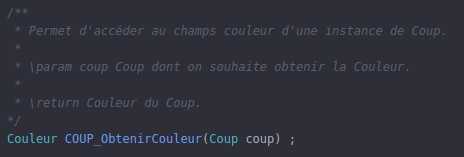
\includegraphics[width=18cm]{./sourcesIMAGES/obtenircouleur.png}
    \caption{La fonction COUP ObtenirCouleur est préfixée par COUP car c’est une action portant sur le type Coup, les commentaires utilisent des balises de Doxygen et le nom de fonction est significatif}
  \end{figure}

  Nous avons utilisé la notation en CamelCase de deux façons différentes dans notre projet. Les fonctions ont des noms avec une majuscule au tout premier mot, tandis que les variables ont une majuscule seulement à partir du second.
